\documentclass{beamer}
\usepackage{listings}
\lstset{
%language=C,
frame=single, 
breaklines=true,
columns=fullflexible
}
\usepackage{blkarray}
\usepackage{subcaption}
\usepackage{url}
\usepackage{tikz}
\usepackage{tkz-euclide} % loads  TikZ and tkz-base
%\usetkzobj{all}
\usetikzlibrary{calc,math}
\usepackage{float}
\newcommand\norm[1]{\left\lVert#1\right\rVert}
\renewcommand{\vec}[1]{\mathbf{#1}}
\usepackage[export]{adjustbox}
\usepackage[utf8]{inputenc}
\usepackage{amsmath}
\usepackage{tikz}
\usepackage{graphicx}
\usetikzlibrary{automata, positioning}
\usetheme{Madrid}
\usecolortheme{whale}
\providecommand{\pr}[1]{\ensuremath{\Pr\left(#1\right)}}
\providecommand{\mbf}{\boldsymbol}
\providecommand{\pr}[1]{\ensuremath{\Pr\left(#1\right)}}
\providecommand{\qfunc}[1]{\ensuremath{Q\left(#1\right)}}
\providecommand{\fn}[1]{\ensuremath{f\left(#1\right)}}
\providecommand{\e}[1]{\ensuremath{E\left(#1\right)}}
\providecommand{\sbrak}[1]{\ensuremath{{}\left[#1\right]}}
\providecommand{\lsbrak}[1]{\ensuremath{{}\left[#1\right.}}
\providecommand{\rsbrak}[1]{\ensuremath{{}\left.#1\right]}}
\providecommand{\brak}[1]{\ensuremath{\left(#1\right)}}
\providecommand{\lbrak}[1]{\ensuremath{\left(#1\right.}}
\providecommand{\rbrak}[1]{\ensuremath{\left.#1\right)}}
\providecommand{\cbrak}[1]{\ensuremath{\left\{#1\right\}}}
\providecommand{\lcbrak}[1]{\ensuremath{\left\{#1\right.}}
\providecommand{\rcbrak}[1]{\ensuremath{\left.#1\right\}}}
\newcommand{\R}{\mathbb{R}}
\newcommand{\C}{\mathbb{C}}
\newcommand{\Int}{\int\limits}
\newcommand{\Sum}{\sum\limits}
\title{\textbf{Research Paper Presentation}}
\subtitle
{\Large{Error Probability for Multilevel Systems in  Presence of Intersymbol Interference and Additive Noise\\} 
                                        \textcolor{yellow}{Michel Nakhla}}  %Author
\author{Suraj Telugu - CS20BTECH11050}
\institute{IITH} 
\date{\today}
\begin{document}
%slide 1 
\begin{frame}
\titlepage
\end{frame}
%slide 2
\begin{frame}{Abstract}
\begin{enumerate}[]
    \item In \textbf{“Performance evaluation of optical fiber transmission systems, by M Nakhla”} a technique for
          evaluation of error probability in fiber-optic communication was proposed
    \item This technique is generalised for Multilevel Digital Systems  
    \item First, We will discuss the prerequisites and previous methods in evaluating error probability
    \item The crux of this method is a \textbf{Minimax Approximation} of 
          cumulative distribution function of additive noise will be explained
    \item Finally, examples and comparisons with previously published techniques are presented along with simulations
\end{enumerate}
\end{frame}
%slide 3
\begin{frame}{Introduction}
\begin{block}{Digital Communication System}
\begin{enumerate}[]
\item \textbf{Primary Objectives} :
\begin{enumerate}[a]
\item Maximize repeater spacing
\item Maintaining a specified error performance
\end{enumerate}
\item Evaluating system performance - Average error probability (BER)
\item Bit error rate(BER) estimated by Computer-aided design(CAD) tools
\end{enumerate}
\end{block}
\begin{block}{Role of CAD Tools}
\begin{enumerate}[]
\item  Estimates BER as a function of specific characteristics of system 
\item  Margin allocation, Sensitivity analysis
\item  Identification of specified components
\item  Cost performance tradeoff
\end{enumerate}
Successful CAD : Efficient and accurate to compute error probability
\end{block}
\end{frame}
%slide 4
\begin{frame}{Introduction}
\begin{block}{Techniques used to estimate Error Probability}
\textbf{Exhaustive Technique :}
\begin{enumerate}[]
\item Evaluating the conditional error probability for each of the possible sequences of data and computing their
      average
\item Average Error Probability $=$ Mean(Conditional Error Probabilities)  
\item Computational cost is highly expensive
\item Limits the number of interfering samples
\end{enumerate}
\textbf{Bounding Error Probability :}
\begin{enumerate}[]
\item Series Expansion Method
\item Gauss Quadrature  
\item New Method : \textbf{Minimax approach} 
\end{enumerate}
\end{block}
\end{frame}
%slide 5
\begin{frame}{Introduction}
\begin{block}{Series Expansion Method}
\begin{enumerate}[]
\item Simple method with less computational cost
\item Slow Convergence
\item Provides oscillating results during channel distortion, increase in Signal to Noise Ratio(SNR) or 
      increase in the number of levels 
\end{enumerate}
\end{block}
\begin{block}{Use of Gaussian Quadrature Rules}
\begin{enumerate}[]
\item More accurate than series expansion
\item Numerical procedure becomes increasingly ill-conditioned as no of moments of R.V representing
      intersymbol interference is increased
\end{enumerate}
\textbf{ILL-Conditioned Problem :} A problem where, for a small change in the independent variables there is a large
change in the dependent variable. 
This means that correct solution to the equation becomes hard to solve.
\end{block}
\end{frame}
%slide 6
\begin{frame}{Introduction}
\begin{block}{Minimax approach}
\begin{enumerate}[]
 \item The proposed Computational algorithm is based on deriving a best approximation(in minmax sense) for CDF of 
       the additive noise
\item This method guarantees that for a given number of moments error in evaluating error probability is minimum 
\end{enumerate}
\end{block}
\begin{block}{Problem Statement}
Digital system to be considered as shown in Figure \eqref{fig.1}. Input to the decision circuit at time 
t is given by 
\begin{align}
y(t) &= \sum_{k = -\infty}^{\infty} a_{k}\,h(t-kT) + n(t)
\end{align}

\end{block}
\end{frame}
%slide 7
\begin{frame}{Problem Statement}
\begin{figure}
    \centering{
    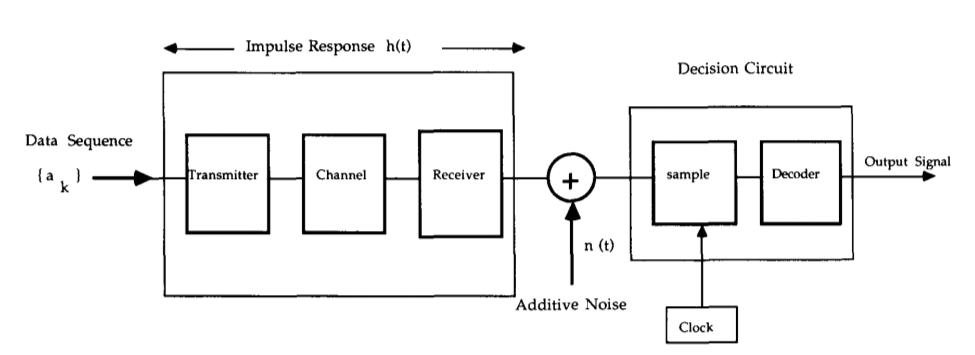
\includegraphics[width=12cm]{DTS_Model.png}}
    \caption{Model of a data transmission system}
    \label{fig.1}
\end{figure}
\end{frame}
%slide 8
\begin{frame}{Problem Statement}
\begin{block}{NOTATIONS}
    \begin{center}
    \begin{tabular}{ |c|c| } 
    \hline
    SYMBOL & DENOTES \\ 
    \hline
    $y(t)$ & Input at Decision Circuit\\ \hline
    $a_{k}$ & Sequence of Random Variables\\ \hline
    $h(t)$ & Impulse Response\\ \hline
    $n(t)$ & Equivalent Additive Noise\\ \hline
    $1/T$ & Bit Rate\\ \hline
    \end{tabular}
    \end{center}
\end{block}
\begin{block}{Calculating Error Probability}
Each $a_{k} \in \{d_{1},d_{2}\} : d_{2}>d_{1}$  with probabilities $p_{1},p_{2}$ respectively,  
Received Signal at decision time $t_{0}$ is given by
\begin{align}
y_{0} &= a_{0}h_{0} + n_{0} + x \label{eqn_2}  \\
y_{0} &= y(t_{0}),\,h_{0} = h(t_{0}),\,n_{0} = n(t_{0})
\end{align}
\end{block}
\end{frame}
%slide 9
\begin{frame}{Problem Statement}
\begin{block}{Calculating Error Probability}
\begin{equation}
x = \Sum_{\substack{k=-\infty \\ k\neq 0}}^{\infty}{a_{k}h(t_{0}-kT)}\;\;\text{(In equation\eqref{eqn_2})}
\end{equation}
Let threshold value of $y_{0}$ be $S$, error probability in the form of conditional probability with respect to
source symbols given as
\begin{align}
P_{e} &= p_{1}\pr{y_{0}>S | a_{0}=d_{1}} + p_{2}\pr{y_{0}<S | a_{0}=d_{2}} 
\end{align}
\begin{multline}
P_{e} = p_{1}\Int_{R}g(x)\brak{1-D(S-x-d_{1}h_{0})} + p_{2}\Int_{R}g(x)D(S-x-d_{2}h_{0}) \label{eqn_6}
\end{multline}
Where $g(x)$,$D(x)$ is PDF and CDF of additive noise in equation\eqref{eqn_6}. $R$ is range of 
definition of $x$
\end{block}
\end{frame}
%slide 10
\begin{frame}{Problem Statement}
\begin{block}{Calculating Error Probability of Multilevel Signals}
For Multilevel Signals $a_{k}$ can take values from $\{\pm 1,\pm 3,\cdots \pm (2L-1)\}$ with equal probabilities
error probability given by 
\begin{align}
P_{e} = K(L)\Int_{R} g(x)\brak{1-D(h_{0}-x)}\,dx \label{eqn_7}
\end{align}
Where $K(L)=2(1-1/2L)$ for pulse amplitude modulation(PAM) system
Equation\eqref{eqn_7} assumes slicing levels $0,\pm 2h_{0},\cdots \pm (2L-2)h_{0}$ and even PDF for additive noise 
\end{block}
\begin{block}{Level Slicing}
An enhancement technique where the Digital Numbers (DN) distributed along the x-axis of an image histogram is divided into a series
of analyst-specified intervals of “slices”.
\end{block}
\end{frame}
%slide 11
\begin{frame}{Problem Statement}
\begin{block}{Special Case for Additive noise Guassian}
\begin{align}
P_{e} &= K(L)\Int_{R} g(x)\,Q\brak{\dfrac{h_{0}+x}{\mu}}\,dx \label{eqn_8} \\
\qfunc{x}  &= \dfrac{1}{\sqrt{2\pi}}\Int_{x}^{\infty}e^{\frac{-w^{2}}{2}}\,dw
\end{align} 
$\mu$ standard deviation of additive noise and $\qfunc{x}$ is Gaussian Q function
\end{block}
\end{frame}
%slide 12
\begin{frame}{Problem Statement}
\begin{block}{General Average Error Probability}
From Equation\eqref{eqn_6}-\eqref{eqn_8} Average error probability is given by
\begin{align}
P_{e} = \Int_{R} f(x)g(x)\,dx \label{eqn_10}
\end{align}
Where PDF $g(x)$ of the intersymbol interference(ISI) is not known unless a direct enumeration of all possible sequences is 
performed,which requires a large amount of computational CPU time
\end{block}
\begin{block}{Intersymbol Interference(ISI)}
This is a form of distortion of a signal, in which one or more symbols interfere with subsequent signals, causing more noise or
delivering a poor output and thus makes communication less reliable
\end{block}
\end{frame}
%slide 13
\begin{frame}{Evaluation of Error Probability (Minimax approach)}
If $f(x)$ is continuous in the interval $\sbrak{-a,a}$ then 
\begin{align}
\Int_{-a}^{+a} f(x)g(x)\,dx \cong \mbf{F^{T} B^{(m)}\;A M^{(m)}} \label{eqn_11}
\end{align}
$\mbf{F}$ is n-dimensional vector which has scaled derivatives of $f(x)$ at $x=0$
\begin{equation}
\mbf{F^{T}} = \sbrak{f(0),\dfrac{f^{(1)}(0)a}{1!},\cdots \dfrac{f^{(n-1)}(0)a^{n-1}}{(n-1)!}}
\end{equation}
$\mbf{M^{(m)}}$, m-dimensional vector $(m\leq n)$ which has scaled derivatives of $g(x)$
\begin{align}
\mathbf{M^{(m)}} = \sbrak{M_{0},\dfrac{M_{1}}{a},\cdots\dfrac{M_{m-1}}{a^{n-1}}}^{T} \\
\text{Where, }\; M_{k} = \Int_{-a}^{a} x^{k}g(x)\,dx
\end{align}
\end{frame}
%slide 14
\begin{frame}{Evaluation of Error Probability (Minimax approach)}
$\mbf{A}=\{a_{i,j}\}$ and $\mbf{B^{(m)}}=\{b_{i,j}^{(m)}\}$ are $(m \times m)$ and $(n \times m)$
\textbf{constant} matrices (independent of $f$,$g$) which are recursively generated 
\null \par \null
\textbf{For a given number of moments and $\mbf{n>>1}$ :} \\
The equation\eqref{eqn_11} is the minimax approximation of \eqref{eqn_10}
and best approximation in Chebyshev sense,of $f(x)$ in the interval $\sbrak{-a,a}$ 
\null \par \null
\begin{block}{Using minimax approach on equation\eqref{eqn_6}}
\begin{align}
P_{e} \cong \sbrak{p_{1}F_{1}^{T} + p_{1}F_{1}^{T}}B^{(m)}\;A M^{(m)} \label{eqn_15}
\end{align}
$\mbf{F_{1},F_{2}}$ contain the scaled derivatives of $\brak{1-D(s-x-d_{1}h_{0})}$ and $D(s-x-d_{2}h_{0})$ 
respectively, $\mbf{M^{m}}$ contains the scaled moments of the ISI
\end{block}
\end{frame}
%slide 15
\begin{frame}{Evaluation of error probability (Minimax approach)}
\begin{block}{Using minimax approach on equation\eqref{eqn_7}}
For 2L-level system, the error probablity is evaluated by 
\begin{equation}
P_{e} \cong K(L)F^{T} B^{(m)}\;A M^{(m)}
\end{equation}
Where $\mbf{F}$ contains scaled derivatives of $\sbrak{1-D(h_{0}-x)}$
\end{block}
\begin{block}{Minmax approach for Gaussian Additive noise}
In equation\eqref{eqn_15}, F contains scaled derivatives given by
\begin{align}
\mbf{F} &= \cbrak{\dfrac{f^{(i)}(0) a^{i}}{i!}} ; \; i\in \cbrak{1,2,\cdots,n} \\
f^{(i)}(0) &= \sqrt{\dfrac{2}{\pi}} \dfrac{(-1)}{\mu}^{i} e^{-\sbrak{\dfrac{h_{0}}{\sqrt{2}\mu}}^{2}} H_{i-1}\brak{\dfrac{h_{0}}{\mu}}
\end{align}
\end{block}
\end{frame}
%slide 16
\begin{frame}{Examples and Comparisons}
\begin{block}{Hermite Polynomial}
$H_{k}(x)$ is a Hermite polynomial of degree k which can be generated using the recursive relation
\begin{align}
H_{k+1}(x) = x H_{k}(x) - k H_{k-1}(x) \\
\text{With } H_{0}(x) = 1 \;,\; H_{1}(x) = x
\end{align}
\end{block}
\begin{block}{Example 1}
Considers the binary PAM transmission, the received pulse is assumed to have the 
form below, For a truncated 11-pulse train approximation
\begin{align}
h(t) &= \dfrac{\sin{(\pi t/T)}}{\pi t/T} \\
\nonumber \text{Sampling time($t_{0}$)} &= 0.2T \; \; \text{Signal to Noise Ratio(SNR)} = 16\;dB
\end{align}
\end{block}
\end{frame}
%slide 17
\begin{frame}{Examples and Comparisons}
\begin{block}{Example 1 simulation data}
\begin{table}[]
    \centering
\resizebox{\columnwidth}{!}{
\begin{tabular}{|c|c|c|c|}
\hline
 \multicolumn{4}{|c|}{Error Probability for a Binary Digital System ($P(e)$)} \\
 \hline
\multicolumn{4}{|c|}{Exhaustive method $P(e)=2.7614\times 10^{-3}$} \\
 \hline
Order of highest moment used  &    Quadrature Rule          &   Series Expansion       & Minmax Approximation      \\ \hline
            4                 &    $3.77\times10^{-5}$      &   $4.2 \times 10^{-6}$   & $2.9758 \times 10^{-3}$   \\ \hline
            6                 &    $8.86\times10^{-4}$      &   $5.98 \times 10^{-5}$  & $2.7650 \times 10^{-3}$   \\ \hline
            8                 &    $2.4\times10^{-3}$       &   $4.71 \times 10^{-4}$  & $2.7573 \times 10^{-3}$   \\ \hline
            10                &    $2.9\times10^{-3}$       &   $2.14 \times 10^{-3}$  & $2.7610 \times 10^{-3}$   \\ \hline
            12                &    $2.8\times10^{-3}$       &   $5.46 \times 10^{-3}$  & $2.7610 \times 10^{-3}$   \\ \hline
            14                &    $2.74\times10^{-3}$      &   $6.56 \times 10^{-3}$  & $2.761446 \times 10^{-3}$  \\ \hline 
            16                &    $2.75\times10^{-3}$      &   $5.06 \times 10^{-4}$  & $2.761442 \times 10^{-3}$  \\ \hline
            18                &   $2.766\times10^{-3}$      &     \centering{-}        & $2.761425 \times 10^{-3}$  \\ \hline
            20                &  $2.7617\times10^{-3}$      &     \centering{-}        & $2.761425 \times 10^{-3}$  \\ \hline
            22                &  $2.7615\times10^{-3}$      &     \centering{-}        & $2.761425 \times 10^{-3}$  \\ \hline
            24                & $2.76164\times10^{-3}$      &     \centering{-}        & $2.761425 \times 10^{-3}$  \\ \hline
\end{tabular}}
 \caption{Example 1}
\label{tab:Table 1}
\end{table}
\end{block}
\end{frame}
%slide 18
\begin{frame}{Simulation Graph - Example 1}
\begin{figure}
 \centering{
    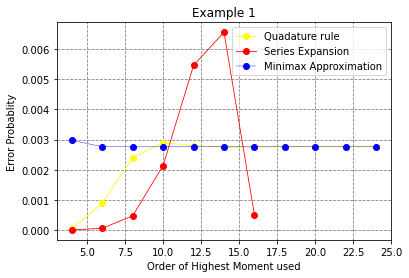
\includegraphics[width=9cm]{Example 1.png}}
    \caption{Error Probability for a Binary Digital System}
    \label{fig.2}
\end{figure}
\end{frame}
%slide 19
\begin{frame}{Examples and Comparisons}
\begin{block}{Conclusions from Table\eqref{tab:Table 1}}
\begin{enumerate}[]
\item Series expansion has low accuracy, provides oscillating results and for moments$>16$ approximation gives
      negative value for error probability
\item Gaussian Quadrature has low accuracy for moments$<6$ but for higher moments it gives accurate results
      but with high computational cost
\item Minimax approximation provides with precise and accurate results with low computational cost
\end{enumerate}
\end{block}
\begin{block}{Example 2}
Consider a four-level PAM signal. The received pulse is given below, for a truncated 5-pulse train
\begin{align}
h(t) = \dfrac{\sin{(\pi t/T)}}{\pi t/T}\;\;\;t_{0} = 0.05T \;\;\; \text{SNR}= 24\;dB
\end{align}
\end{block}
\end{frame}
%slide 20
\begin{frame}{Examples and Comparisons}
\begin{block}{Example 2 simulation data}
\begin{table}[]
    \centering
\resizebox{0.62\columnwidth}{!}{
\begin{tabular}{|c|c|}
\hline
 \multicolumn{2}{|c|}{Error Probability for a Four level System ($P(e)$)} \\
 \hline
\multicolumn{2}{|c|}{Exhaustive method $P(e)=5.2\times 10^{-7}$} \\
 \hline
Order of highest moment used  &    Minimax Approximation        \\ \hline
            8                 &    $1.4\times10^{-7}$          \\ \hline
            10                &    $2.7\times10^{-7}$           \\ \hline
            12                &    $4.0\times10^{-7}$            \\ \hline
            14                &    $5.0\times10^{-7}$            \\ \hline
            16                &    $5.27\times10^{-7}$            \\ \hline
            18                &    $5.26\times10^{-7}$           \\ \hline 
            20                &    $5.21\times10^{-7}$            \\ \hline
            22                &    $5.199\times10^{-7}$            \\ \hline
            24                &    $5.204\times10^{-7}$           \\ \hline
            26                &    $5.205\times10^{-7}$            \\ \hline
            28                &    $5.204\times10^{-7}$             \\ \hline
            30                &    $5.204\times10^{-7}$             \\ \hline
\end{tabular}}
 \caption{Example 2}
\label{tab:Table 2}
\end{table}
\end{block}
\end{frame}
%slide 21
\begin{frame}{Simulation Graph - Example 2}
\begin{figure}
 \centering{
    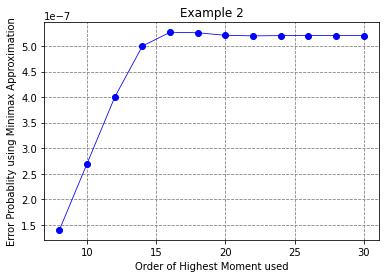
\includegraphics[width=9cm]{Example 2.png}}
    \caption{Error Probability for a Four Level System}
    \label{fig.3}
\end{figure}
\end{frame}
%slide 22
\begin{frame}{Examples and Comparisons}
\begin{block}{Example 3}
 This example considers a binary system with non-Gaussian additive noise. The received pulse is given by
 \begin{align}
h(t) = \dfrac{\sin{(\pi t/T)}}{\pi t/T}\;\;\;t_{0} = 0.2T \;\;\; \text{SNR}= 24\;dB
 \end{align}
Additive noise is assumed to be Cauchy distributed with PDF 
\begin{align}
\phi(x) = \dfrac{10^{-2}}{x^{2}+10^{-4}}
\end{align}
For a truncated 11-pulse train, Table 3 shows the minimax approach
\end{block}
\end{frame}
%slide 23
\begin{frame}{Examples and Comparisons}
\begin{block}{Example 3 simulation data}
\begin{table}[]
    \centering
\resizebox{0.8\columnwidth}{!}{
\begin{tabular}{|c|c|}
\hline
 \multicolumn{2}{|c|}{Error Probability for a Binary System ($P(e)$)} \\
\multicolumn{2}{|c|}{With Non-Gaussian Additive Noise} \\
 \hline
Order of highest moment used  &    Minimax Approximation        \\ \hline
            2                 &    $3.19\times10^{-3}$          \\ \hline
            4                 &    $4.17\times10^{-3}$           \\ \hline
            6                 &    $4.115\times10^{-3}$            \\ \hline
            8                 &    $4.119\times10^{-3}$            \\ \hline
            10                &    $4.118\times10^{-3}$            \\ \hline
            12                &    $4.119\times10^{-3}$           \\ \hline 
            14                &    $4.119\times10^{-3}$            \\ \hline
            16                &    $4.119\times10^{-3}$            \\ \hline
\end{tabular}}
 \caption{Example 3}
\label{tab:Table 3}
\end{table}
\end{block}
\end{frame}
%slide 24
\begin{frame}{Simulation Graph - Example 3}
\begin{figure}
 \centering{
    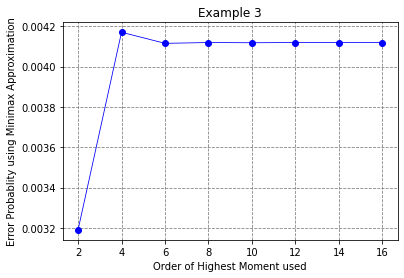
\includegraphics[width=9cm]{Example 3.png}}
    \caption{Error Probability for a Binary System with Non-Gaussian Additive Noise}
    \label{fig.4}
\end{figure}
\end{frame}
%slide 25
\begin{frame}{Conclusion}
\begin{block}{Computational Cost}
\begin{enumerate}[]
\item CPU time required to obtain the results above examples using minimax approximation was under 
      0.4 s on IBM3081KX
\end{enumerate}
\end{block}

\begin{block}{Conclusions from Results}
\begin{enumerate}[]
\item Series expansion works for small range of moments, though Gaussian Quadrature seems accurate
      its computational cost is high and numerical procedure is ill conditioned
\item Minmax approach provides accurate and precise results for a wide number of moments with low 
      computational cost 
\item This method guarantees that for a number of moments the error in evaluating error probability is 
      minimum
\item The additive noise is not constrained to be Gaussian function
\end{enumerate}
\end{block}
\end{frame}
%slide 26 (Thank you slide)
\begin{frame}
   \centering
    \textcolor{blue}{\Huge{\textbf{THANK YOU}}}
 \begin{figure}
 \centering{
    
\includegraphics[width=3cm]{logo.png}}
    \label{logo}
\end{figure}  
\end{frame}
\end{document}